\documentclass{article}
\usepackage[latin1]{inputenc}    
\usepackage[T1]{fontenc}
\usepackage[french]{babel}
\usepackage{graphicx}
\newcommand\tab[1][1cm]{\hspace*{#1}}
\usepackage{geometry}
\geometry{hmargin=3.45cm,vmargin=3cm}
\usepackage{color}
\definecolor{myblue}{rgb}{0.15, 0.15, 0.8}

\begin{document}

\newpage
\title{ Manuel d'utilisation }
 
\maketitle

\newpage
Lors de l'utilisation de l'application une page s'ouvre � afin de pouvoir faire ses manipulations. Un menu est � la port�e : comme le montre la figure1.
\begin{center} 
			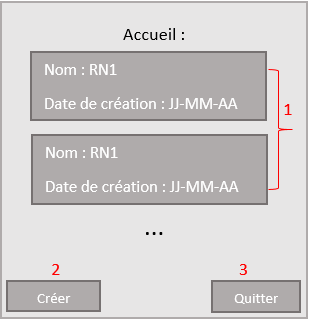
\includegraphics[height=244, width=300]{acceuil.png}
		\end{center}
figure1

\begin{itemize}
	\item S�lectionner (1)  un parmi d'autres r�seaux de neurones d�j� cr��s pr�alablement. En choisir un puis cliquer dessus, une page manipulation R�seau s'ouvrira figure 2. 
	\item Cliquer sur le bouton cr�er (2) pour cr�er un nouveau r�seau de neurones. Une page cr�ation r�seau de neurones s'ouvrira  figure3.
	\item cliquer sur le bouton Quitter (3) pour quitter l'application.
\end{itemize}

\begin{center} 
			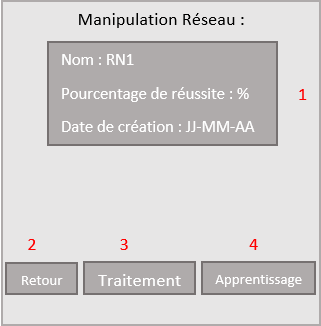
\includegraphics[height=244, width=300]{manip.png}
		\end{center}
figure2

\begin{itemize}
	\item(1) Affichage des informations sur le r�seau de neurones.
	\item cliquer sur le bouton Traitement (3) une page traitement d'images s'ouvrira : comme le montre la figure4.
	\item cliquer sur le bouton Apprentissage (4) lancera l'apprentissage du r�seau de neurones, un deuxi�me clique sur le bouton arr�tera l'apprentissage.
	\item cliquer sur le bouton Retour (2) fait retour � la page d'accueil Figure 1. 
\end{itemize}

\begin{center} 
			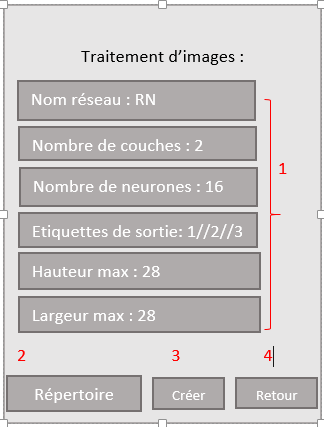
\includegraphics[height=244, width=300]{creation.png}
		\end{center}
figure3

\begin{itemize}
	\item (1) remplir les champs avec les bons param�tres du r�seau
	\item cliquer sur le bouton r�pertoire (2) pour choisir un r�pertoire d'images utile pour l'apprentissage.
	\item cliquer sur le bouton cr�er (3) pour valider les informations et se diriger vers la page manipulation r�seau figure2.
	\item cliquer sur le bouton Retour(4) pour retourner � la page d'accueil figure1
\end{itemize}

\begin{center} 
			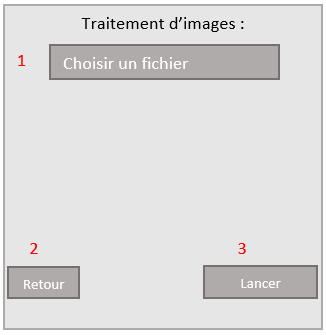
\includegraphics[height=244, width=300]{traitement.png}
		\end{center}
figure4

\begin{itemize}
	\item cliquer sur le bouton retour pour revenir � la page manipulation R�seau figure2.
	\item cliquer sur le bouton choisir fichier (1) pour pouvoir s�lectionner l'image � analyser : comme le montre la figure ci-dessous.
\end{itemize}

\begin{center} 
			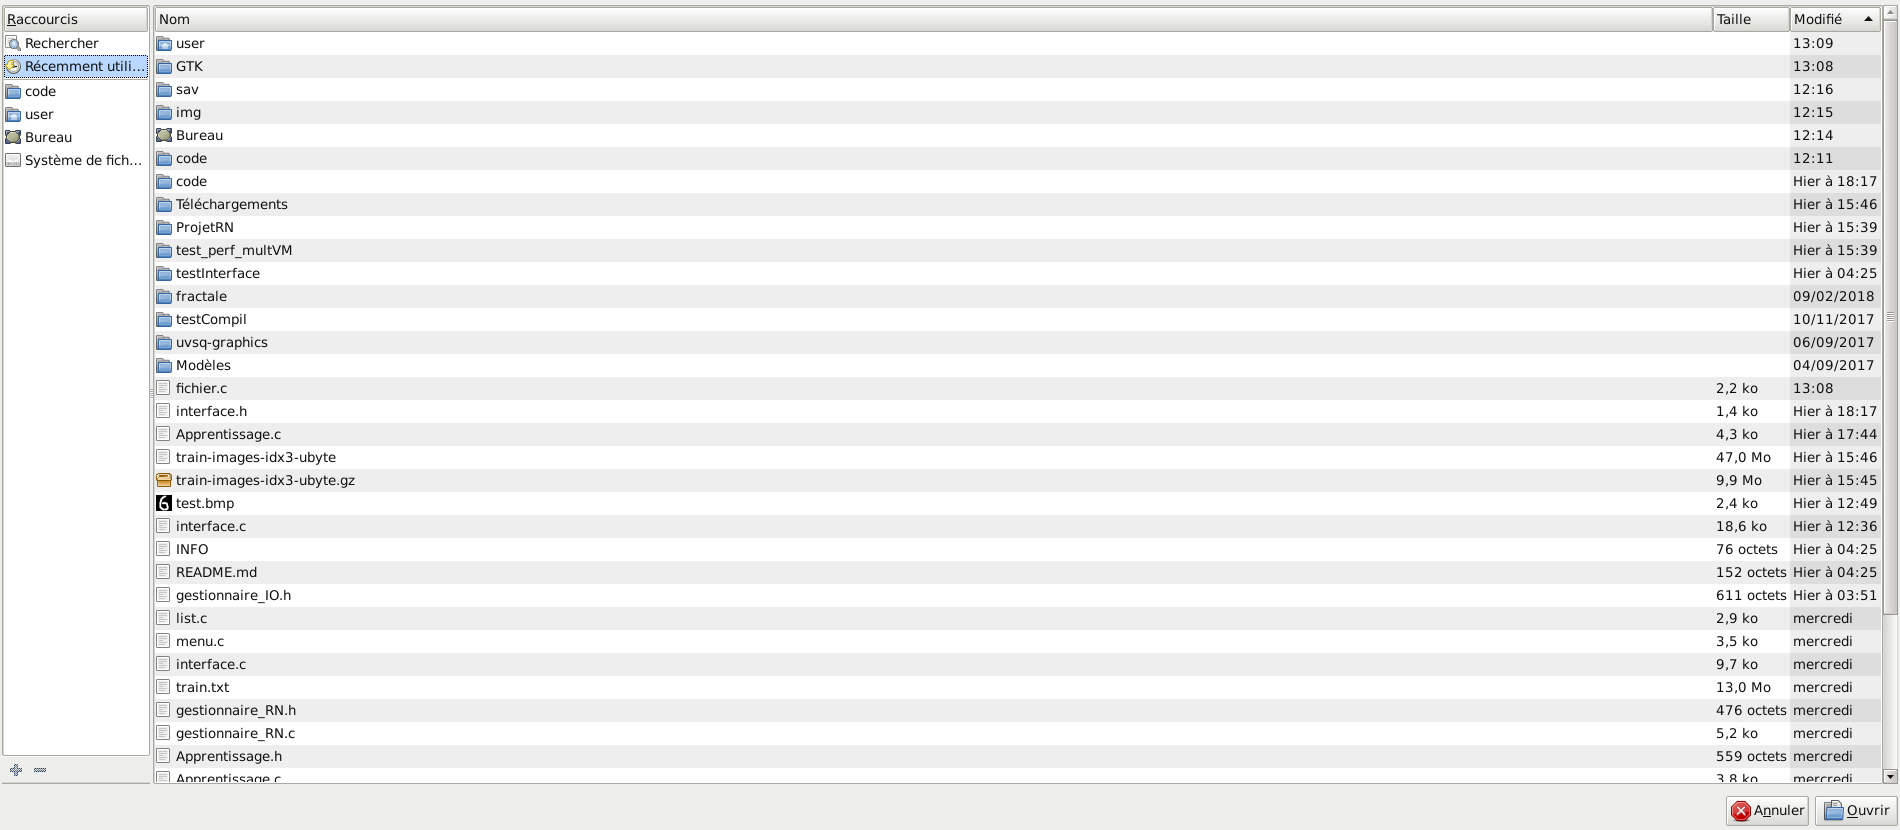
\includegraphics[height=244, width=300]{cap_fichier.png}
		\end{center}

\begin{itemize}
	\item cliquer sur ouvrir pour valider le choix du fichier.
	\item cliquer sur annuler pour annuler et quitter la page.
	\item cliquer sur le bouton Lancer (3) ouvrira la page Top3 des r�sultats figure5. 

\end{itemize}

\begin{center} 
			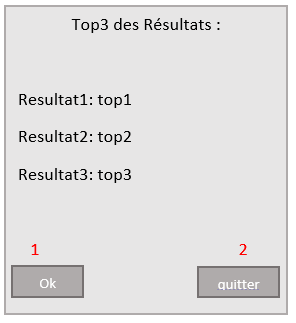
\includegraphics[height=244, width=300]{top_res.png}
		\end{center}
figure5

\begin{itemize}
	\item cliquer sur le bouton ok (1) retour � la page traitement d'image figure4.
	\item cliquer sur le bouton quitter (2) pour quitter l'application.
\end{itemize}

\end{document}